Neural networks created and deployed in mission critical domains must demonstrate high confidence in their predictions. However, without appropriate training data, it is impossible to evaluate the accuracy of the model. In addition, without considering edge cases and other special scenarios which may or may not be infrequent, the neural networks cannot be trained to handle such cases and predict accurately when encountering such scenarios. Furthermore, in high-dimensional input data applications such as image classification, required patterns cannot be easily captured by the available training data set due to its high-dimensional nature which could result in the above situations quite easily. Manifold-based test generation is a technique which provides a means to capture the necessary patterns such that the neural network can learn these patterns in a low-dimensional manifold space. This is achieved by projecting the data points from a high-dimensional input space to a low-dimensional space. The approach uses a Conditional Variational Autoencoder (CVAE) to capture the manifold space which is then utilized to generate novel fault-revealing test cases. Please note that a unique feature of this approach is that these test cases are generated along with the labels. Based on our understanding, the resulting fault-revealing test cases can be utilized in two ways: 1) to create a test suite which can evaluate the performance of the neural network, 2) to include the fault revealing test cases as part of the training set such that the neural network performance and accuracy can be improved.

\begin{figure}[h]
%	\vspace{-5mm}
	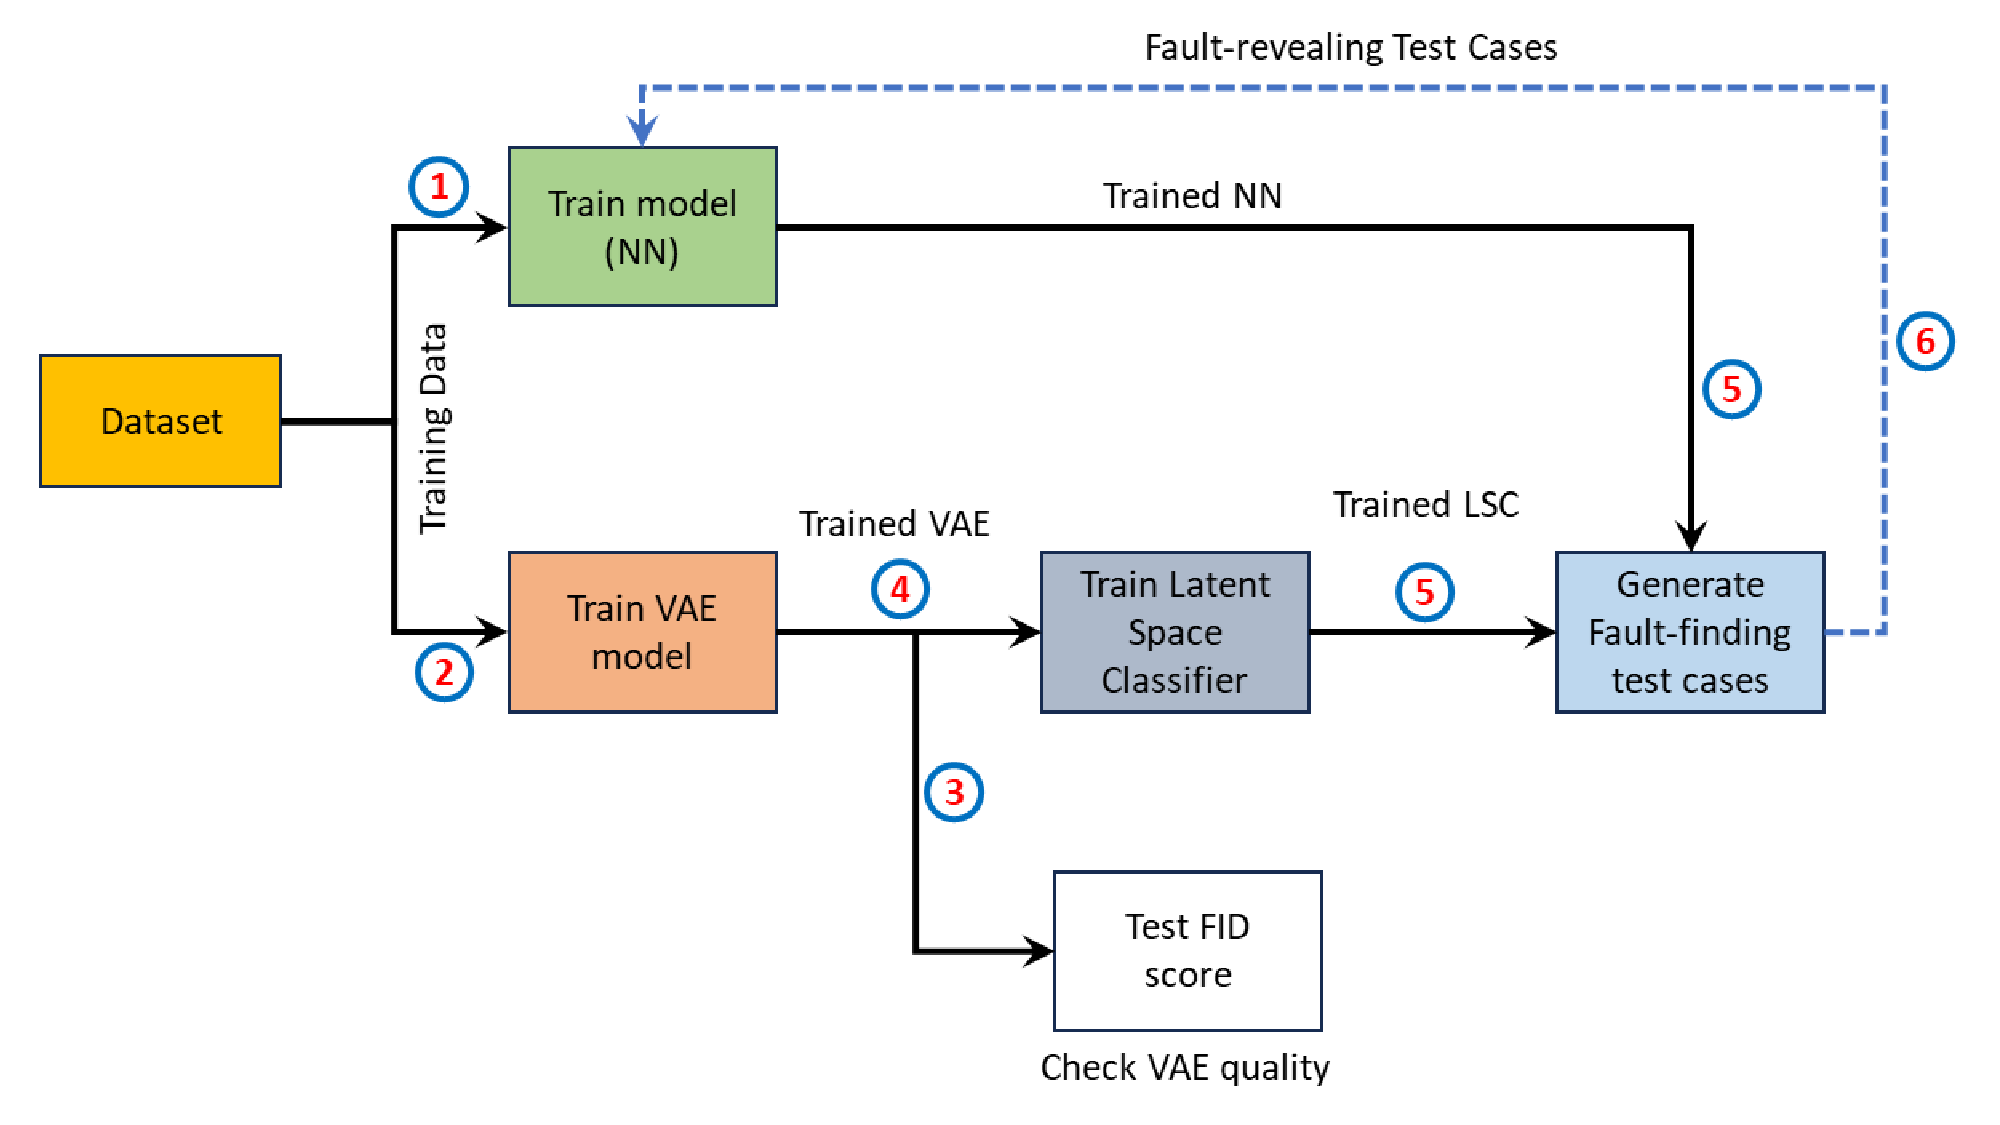
\includegraphics[width=\linewidth]{Fig/manifold_workflow.pdf}
%	\vspace{-20mm}
	\caption{Manifold-Based Test Generation Workflow.}
	\label{fig:manifold_workflow}
\end{figure}

Figure~\ref{fig:manifold_workflow} shows the workflow of the manifold based test generation tool. At first, the neural network is trained using the training data set as shown in Figure~\ref{fig:manifold_workflow} (step 1). The trained neural network can be evaluated for its performance using a separate testing data set which is not shown in this workflow. Next, a trained VAE is generated by using the same training data set which is used for the neural network (step 2). Once the trained VAE model is developed, it can then be used to train the Latent Space Classifier (LSC) as shown in Figure~\ref{fig:manifold_workflow} (step 4). Please note, if needed the user can evaluate the quality of the trained VAE by measuring its FID score (step 3). The closer the FID score to zero, the better the trained VAE is assumed to be. Please note, this step can also be performed before training the LSC. The LSC is responsible to learn the manifold space. Further, in order to generate fault-revealing test cases from the manifold space, the trained neural network and the LSC are passed as an input to the test generation algorithm (step 5). The algorithm then selects the test cases from the manifold space which includes the label and evaluates it using the neural network. If the neural network mis-predicts the output, the test case is considered as a fault-revealing test. The algorithm is able to generate the desired number of faulty test cases. The test cases can be utilized as part of the training data set to re-train the original neural network (step 6). Please note that this step is represented using dashed line because this feature is currently not provided by the tool.

\subsection{Tool evaluation:} We evaluated the tool on MNIST dataset and followed the workflow as describe above in Figure 9. Fault revealing test cases can be generated by following various algorithms, but the two types of algorithms utilized in our evaluation are the random test generation and the search-based test generation. We have shown the results for both of them below. 

\begin{itemize}
	\item \textit{Random Test Case Generation:} Using this test generation algorithm the desired number of test cases are generated. However, not all test cases may be fault-revealing. Figure~\ref{fig:random} represents generation of 50 random test cases. Out of 50 test cases, only 5 of these test cases were identified as fault-revealing. These test cases are shown with different color boxes in Figure 10. From Figure~\ref{fig:random}, it is impossible to understand the reasoning behind the selection of fault-revealing test cases, meaning one cannot tell whether the tool identified the test cases correctly or not. Hence, a visual representation can provide a better insight. Therefore, we have generated visual representation for each of the test cases shown in Figure~\ref{fig:random}. This visual representation is shown in Figure~\ref{fig:random_visual}. Again, each fault- revealing test case is color coded for ease of understanding. 
	\begin{figure}[h]
		%	\vspace{-5mm}
		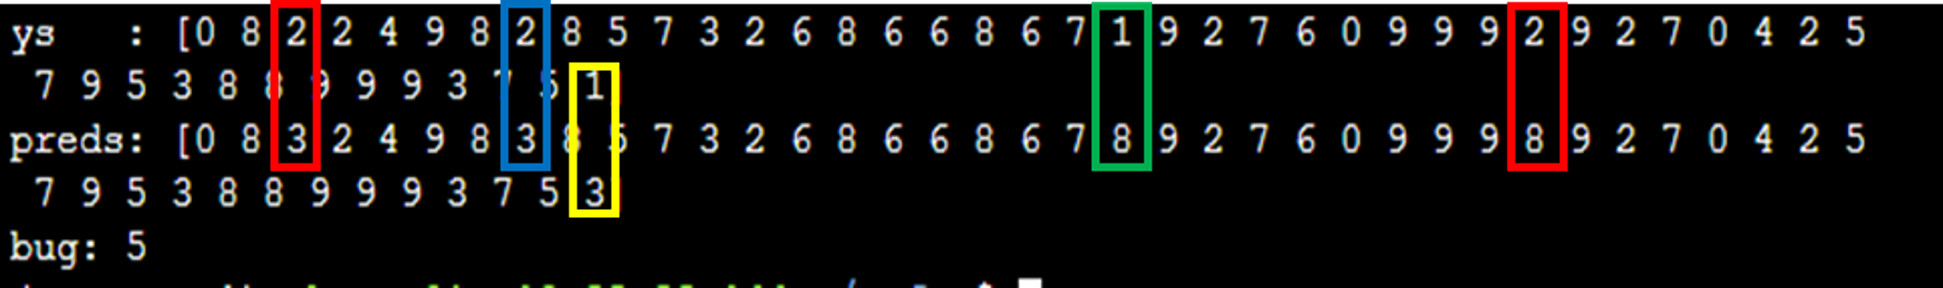
\includegraphics[width=\linewidth]{Fig/random.png}
		%	\vspace{-20mm}
		\caption{Randomly generated test cases.}
		\label{fig:random}
	\end{figure}

	\begin{figure}[h]
		%	\vspace{-5mm}
		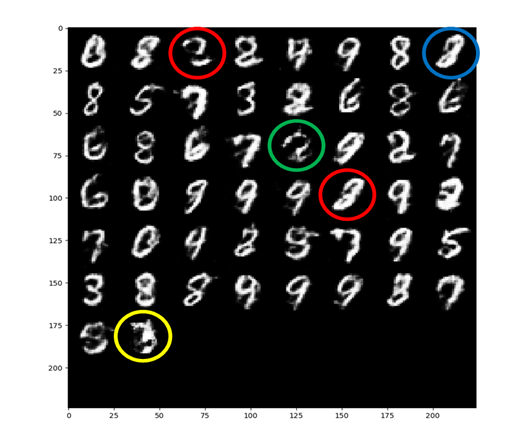
\includegraphics[width=\linewidth]{Fig/random_visual.png}
		%	\vspace{-20mm}
		\caption{Visual representation of randomly generated test cases.}
		\label{fig:random_visual}
	\end{figure}
	\item \textit{Search-Based Test Case Generation:}  Using this test generation algorithm, all the generated test cases are fault-revealing. Figure~\ref{fig:search-based} represents generation of 15 search-based test cases. As shown in Figure~\ref{fig:search-based}, all of the 15 test cases were fault-revealing and they are shown in different color boxes for clarity. Figure~\ref{fig:search_visual} shows the visual representation of each of these fault-revealing test cases. Again, each of these fault-revealing test cases are color coded for ease of understanding.
	\begin{figure}[h]
		%	\vspace{-5mm}
		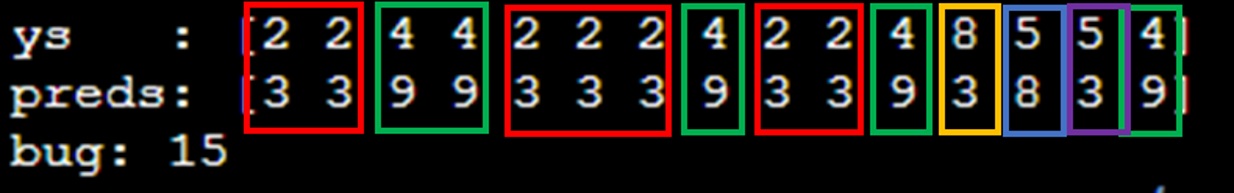
\includegraphics[width=\linewidth]{Fig/search-based.png}
		%	\vspace{-20mm}
		\caption{Search-based generated test cases.}
		\label{fig:search-based}
	\end{figure}

	\begin{figure}[h]
		%	\vspace{-5mm}
		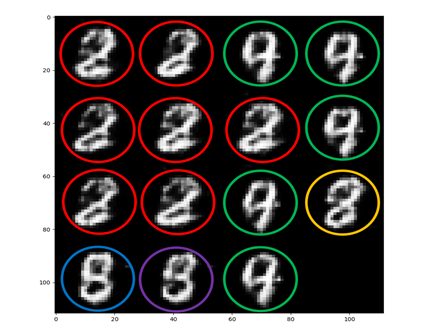
\includegraphics[width=\linewidth]{Fig/search_visual.png}
		%	\vspace{-20mm}
		\caption{Visual representation of search-based generated test cases.}
		\label{fig:search_visual}
	\end{figure}
\end{itemize}
\subsection{Tool Limitations:} Based on our evaluation, the tool provides a unique mechanism to generate fault-revealing test cases for high-dimensional data set. However, the tool still has the following limitations:
\begin{itemize}
	\item The generated fault revealing test cases require manual inspection to be considered as part of the training test suite to improve prediction accuracy. As seen from above figures (Figures 11 and 13), it is obvious that some of the predictions and their visual representations do not match and hence require a manual step to analyze the generated test cases. This could become a significant bottleneck when generating large number of fault-revealing test cases. An automated approach to address this issue would make the tool significantly useful. 
	\item The tool was developed as a prototype to demonstrate the proof of concept and still requires several updates to completely become usable in this space. For instance, the algorithm for search-based test generation was modified slightly to capture only fault-revealing test cases. 
	\item The tool is currently capable to work with MNIST, CIFAR, FASHION, and EMNIST data sets. To use other data sets as inputs, minor tool modification is required such that the tool can handle these new data sets appropriately.
	\item The approach works on high-dimensional data sets, however, for low-dimensional classification problems the tool is unable to handle the data sets appropriately. We believe the approach is sound and should be easily applicable to low-dimensional classification problems. This could easily enable even the neural networks in other classification problem domains to acquire better accuracy. However, currently the tool is unable to handle low-dimensional training data sets and require modification. The extent of modification is not evaluated as part of our process.
\end{itemize}
